\chapter{Introduction}\label{chap:intro}

Quantitative trait locus (QTL) mapping in model organisms is a form of genetic association that has successfully identified genetic variants associated with medically-relevant phenotypes, including but certainly not limited to these examples in rodents: muscle malformation \citep{Hartmann2008, Kelly2013}, cocaine response \citep{Kumar2013}, asthma \citep{Kelada2016,Donoghue2017}, diabetes \citep{SolbergWoods2010,SolbergWoods2012,Keele2017}, and drug response in liver disease \citep{Mosedale2017}. Compared with epidemiological studies of naturally occurring human populations, sometimes referred to with the more general term genome-wide association studies (GWAS) \citep{Mccarthy2008,Teslovich2010,Ripke2014}, crosses of organisms allow for reduced population structure, better control of unobserved environmental factors, and more extensive or invasive phenotyping of samples than is possible with humans. 

Traditionally experimental crosses involved two inbred strains as founders or parents, which can be referred to as bi-parental crosses. Recently, experimental populations in which individuals descend from more than two inbred founder strains, or multiparental populations (MPP), have been developed in a number of model organism systems. These populations, particularly replicable ones, act as rich reservoirs of genetic variants and phenotypic variability that provide the raw material that investigators must sift through for interesting biology relating to their system and model. Their additional complexity also pose unique statistical challenges, for which specialized and bespoke analytical methods could more effectively and efficiently draw insights and inferences. This dissertation is organized into two main topics relating to:
\begin{enumerate} 
	\item Experimental design approaches designed around MPP data and related experiments.
	\item Genetic association approaches for MPP data and related analyses.
\end{enumerate}
Together these sections provide novel advancements in the use of MPP data, both towards the design of experiments and the genetic association analyses, which will allow for these resources to be more effectively utilized. Examples and analyses will generally focus on rodent models, primarily laboratory mice. However, these organisms are not fundamental to the methodology, which could have application to any organism with an MPP. Prior to describing the projects that make up this dissertation in detail, background information will be presented on the various forms of experimental populations, both to provide context and justification for this work.

\section{Experimental populations}

This work generally focuses on studies, that at least in part, seek to associate positions in the genome, or more ideally, genes or variants with phenotypes, primarily within experimental populations, particularly MPP. Genetic association studies fundamentally require the genomes amongst the study samples to be randomized at loci across the genome, thus allowing the effect at one position to be separated from the effect at another. When this randomization is flawed, loci that are not physically linked can become correlated, representing non-syntenic associations, and possibly result in false positive associations. This is the process which underlies population structure, in which genetic drift and non-random mating create the non-syntenic associations that correlate to some extent with unobserved population factors. Whereas population structure must be recognized and accounted for in observational epidemiological populations of humans \citep{Devlin1999,Hoffman2013}, the breeding design in experimental populations of organisms can greatly minimize the issue, as well as strongly controlling other influential factors, resulting in individuals with more perfectly randomized genomes. Alternatively, such individuals can be referred to as exchangeable. It is also important to acknowledge that population structure, and other unobserved confounders, can still occur in experimental populations, and is indeed likely with certain breeding and experimental designs. Still, the potential to have a more ideally controlled population is an appealing feature for using experimental populations as opposed to observational ones.

\subsection{Genetic reference populations}

One useful form of experimental population are collections, or panels, of inbred lines or strains, which began to be developed in full force in the early 20\textsuperscript{th} century in a number of organisms, including the mouse \citep{Casellas2011}. An inbred animal results from multiple generations of inbreeding through sib-sib matings, and are predominantly homozygous at positions across the genome. Whereas the inbred state can be challenging to animals and result in line extinctions \citep{Shorter2017}, plant models can be more amenable, particularly with self-pollinators \citep{Allard1999}, and even cross-pollinators \citep{RobsaShuro2017}. These panels provide researchers a renewable source of replicable genomes, ignoring \textit{de novo} mutations and genetic drift \citep{Keane2011}, and powerfully minimize external sources of error outside of genetic effects specific to the strains. Phenotype surveys across a panel of inbred strains represent stable references within model organism systems \citep{Phillippi2014,Rasmussen2014,McMullan2016,Roberts2018}. For these reasons, inbred panels represent a class of experimental population, the genetic reference population (GRP), primarily providing stable, replicable genomes and phenotypes. For QTL mapping to be possible, the genomes of a population must be randomized through recombination events in meiosis is necessary, thus leading to experimental crosses of inbred strains. 

\subsection{Bi-parental populations}

The simplest experimental crosses involve two strains, which will be referred to as bi-parental crosses or populations \citep{Broman2001}. The simplest bi-parental crosses are F2 intercrosses and backcrosses (BC), which will be discussed in \textbf{Chapter \ref{chap:didact}}, in which only a single generation of genetic recombination occurs between the parental haplotypes, resulting in mapping populations with little population structure but poor mapping resolution. The mapping resolution can be improved through additional generations of intercrosses, often referred to as advanced intercross lines (AIL) \citep{Darvasi1995,Parker2011a,Parker2012,Parker2014}, though population structure can become an issue. These previous bi-parental experimental populations are all outbred and non-replicable. GRP populations that can also function as mapping populations are possible through the development of recombinant inbred (RI) lines or strains, as well as their intercrosses (RIX) \citep{Zou2005}, which are particularly common in plants \citep{Lister1993, Mansur1996, Monforte2000}, though also in mice, such as the BXD lines \citep{Peirce2004,Carbonetto2014}, in which inbreeding generations follow the initial outbreeding generations as in F2 crosses or BC until an inbred state is established, resulting in individuals with genomes that are both inbred and mosaics of the two parental haplotypes. These forms of experimental populations are powerful genetic tools, though they are generally constrained in terms of the overall genetic variation phenotypic variability they can possess from the natural populations from which they descend. Simplified visual representations of these bi-parental populations are in \textbf{Figure \ref{fig:intro_biparental_crosses}}.

\begin{figure}
\centering
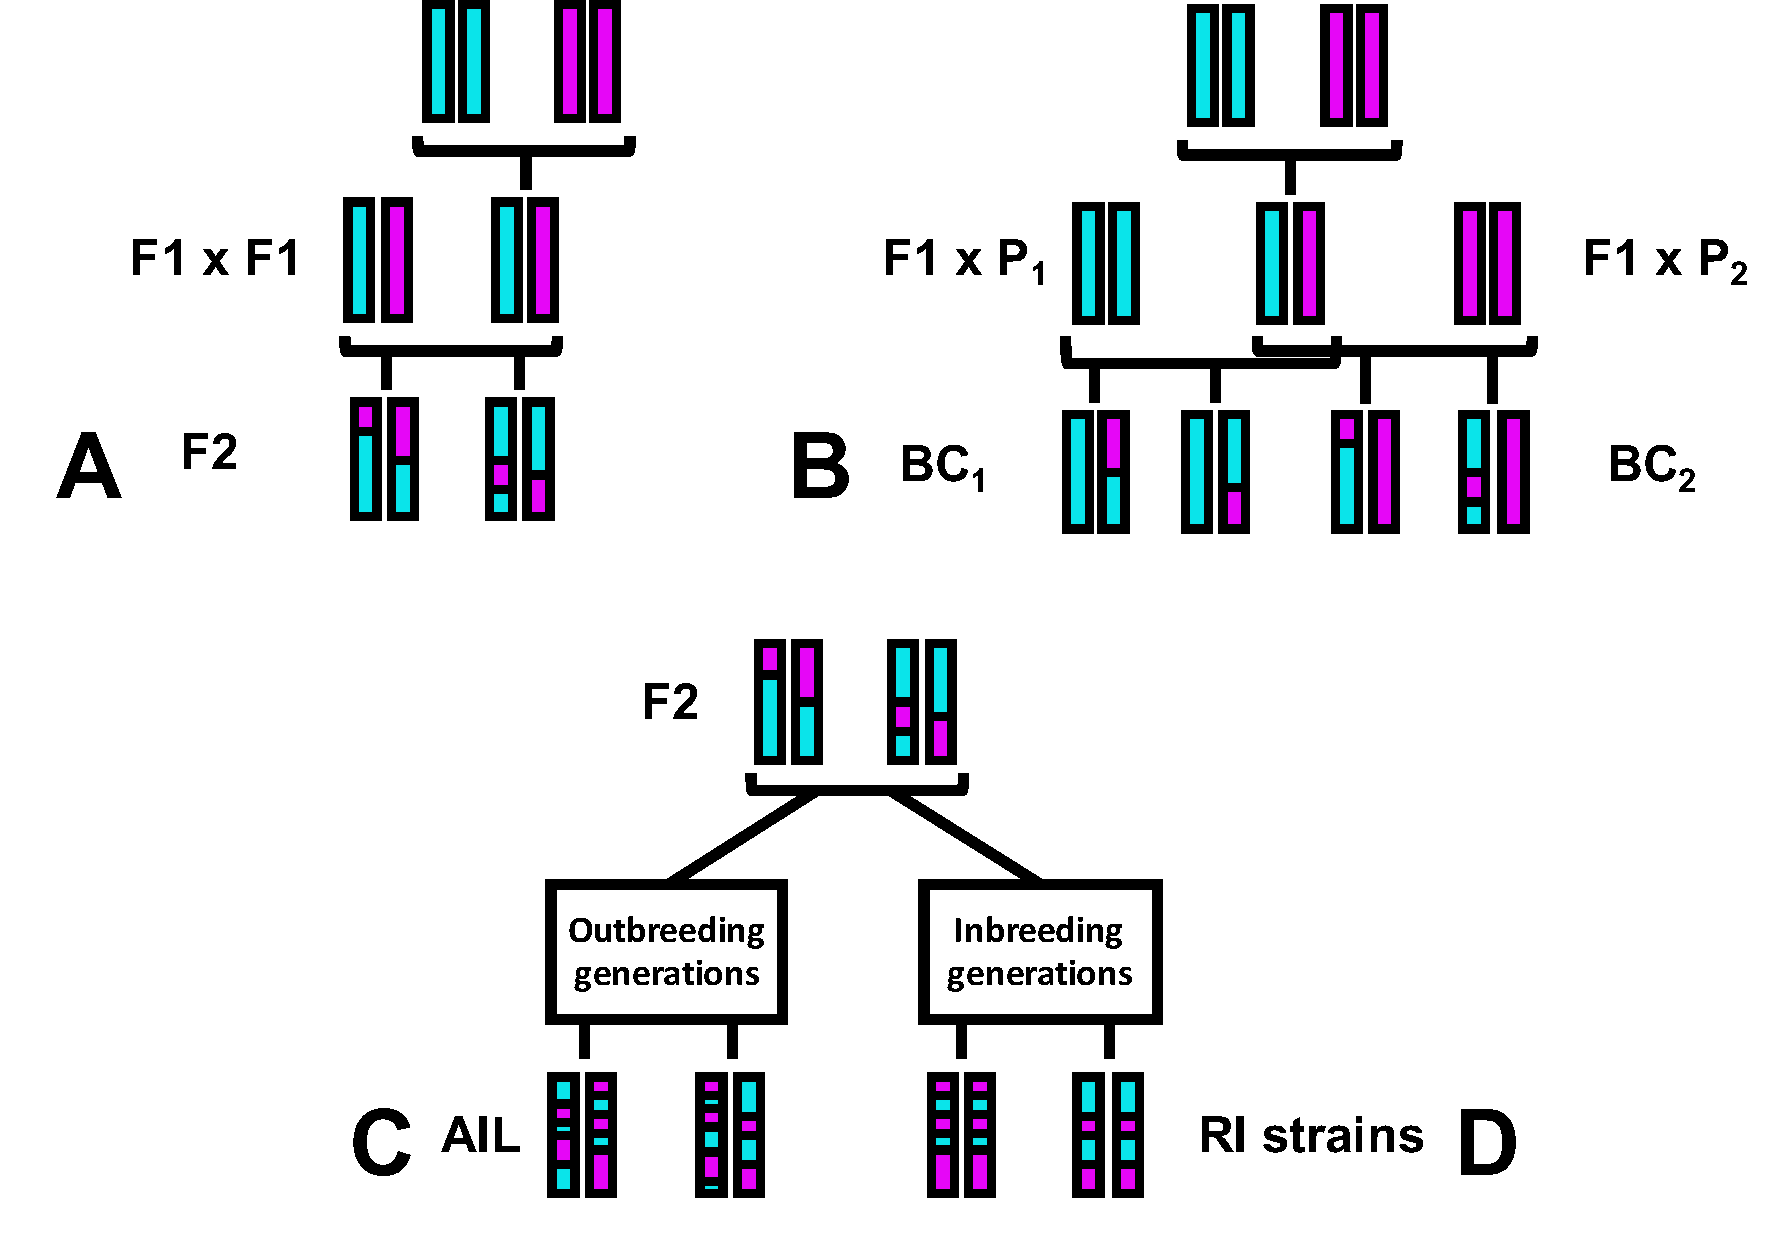
\includegraphics[width=0.8\textwidth, trim={0in 0in 0in 0in}, clip]{figures/1-introduction/crosses_for_dissertation_intro.pdf}
\caption[Simplified bi-parental populations]{Simplified representations of F2 (A), BC (B), AIL (C), and RI strains (D). Each genome is simplified to a single pair of chromosomes, colored with respect to parental haplotypes. The F2, BC, and AIL represent outbred populations. The BC is unique in that at any given locus, only two potential genetic states are observed, rather than three. The RI strains are inbred and replicable, and thus as a panel, represent a GRP. Although these populations are powerful tools for genetic experiments, they are constrained in terms of their genetic variation, as only two founder haplotypes are present. \label{fig:intro_biparental_crosses}}
\end{figure}


\subsection{Multiparental populations}

MPP address this issues of reduced genetic variation in bi-parental populations by incorporating more inbred strains, and thus likely genetic variation, into the populations. A practical challenge involved in the development of MPP is the greater complexity in breeding design; ideally additional lines of inheritance are incorporated in such a way as to avoid population structure as well as maintain balance in terms of founder contributions. 

\subsubsection{Heterogeneous Stock}

Heterogeneous stock (HS) populations in mice \citep{Valdar2006a} and rats \citep{Hansen1984} represent outbred MPP that, due to additional generations of recombinations through outbreeding, have finer mapping resolution. Alternatively, due to the rotational breeding design used, the HS can have greater levels of population structure and founder allele frequency imbalances. These populations can be viewed as an MPP analogue to the bi-parental AIL. HS rat data will be analyzed and discussed in \textbf{Chapters \ref{chap:mi}} and \textbf{\ref{chap:hs_rats}}. As outbred populations, the HS genomes are not replicable, and as such, are not GRP. Recently multiparental genetic reference populations (MPGRP) have been developed in a number of animal and plant models, which bring together the powerful experimental control of panels of inbred strains and the increased genetic diversity of MPP.

\subsubsection{Collaborative Cross and related populations}

MPGRP represent an MPP generalization of bi-parental RI strains and their intercrosses. The Collaborative Cross (CC) \citep{Churchill2004,Hall2012,Srivastava2017}, which will be a focus in \textbf{Chapters \ref{chap:sparcc}}, \textbf{\ref{chap:mi}}, and \textbf{\ref{chap:mediation}}, is an multiparental panel of RI strains in mouse, descended from five traditional inbred strains (A/J, C57BL/6J, 129S1/SvImJ, NOD/LtJ, NZO/H1LtJ) and three wild derived strains (CAST/EiJ, PWK/PhJ, WSB/EiJ), representing three subspecies of the house mouse, \textit{Mus musculus}, and thus collectively possessing a high level of genetic variation \citep{Yang2007,Yang2011}, particularly in comparison to bi-parental populations. Alhough subspecies incompatibilities \citep{Shorter2017} limited the number of strains produced, the CC, and its incipient lines, have been a valuable tool for QTL mapping \citep{Aylor2011, Phillippi2014,Kelada2016,Mosedale2017,Donoghue2017}. The CC is also a source of better murine models of human disease, likely the result of interesting allelic combinations being fixed across the genome, for example, of colitis \citep{Rogala2014}, ebola infection \citep{Rasmussen2014}, and West Nile Virus infection \citep{Graham2015}.

Related MPP have developed out of the CC. The CC F1 intercrosses (CC-RIX) \citep{Rasmussen2014,Graham2015} allow for replicable outbred genomes, which generally produce more robust progeny, representing large scale heterosis \citep{Birchler2006}, and thus better approximating natural populations. Similarly, the Diversity Outbred stock (DO) \citep{Churchill2012,Svenson2012,Gatti2014} represents an outbred population that shares the same founders as the CC, sacrificing replicability but providing fine scale mapping resolution with relatively little population structure. These related populations have the potential to be jointly analyzed, or used to replicate or confirm findings amongst one another, as was done in \cite{Chick2016} in which allele effects at QTL detected in the DO were confirmed in the CC. Together these populations provide a strong foundation for systems genetics in mouse models. MPP and MPGRP have been developed in other organisms, though characteristics vary in terms of number of founder strains, number of resulting RI strains, and breeding design. Simplified representations of the CC and the DO together and the HS are presented in \textbf{Figures \ref{fig:intro_mpp_crosses}} and \textbf{\ref{fig:hs_cartoon}} respectively.

\begin{figure}
\centering
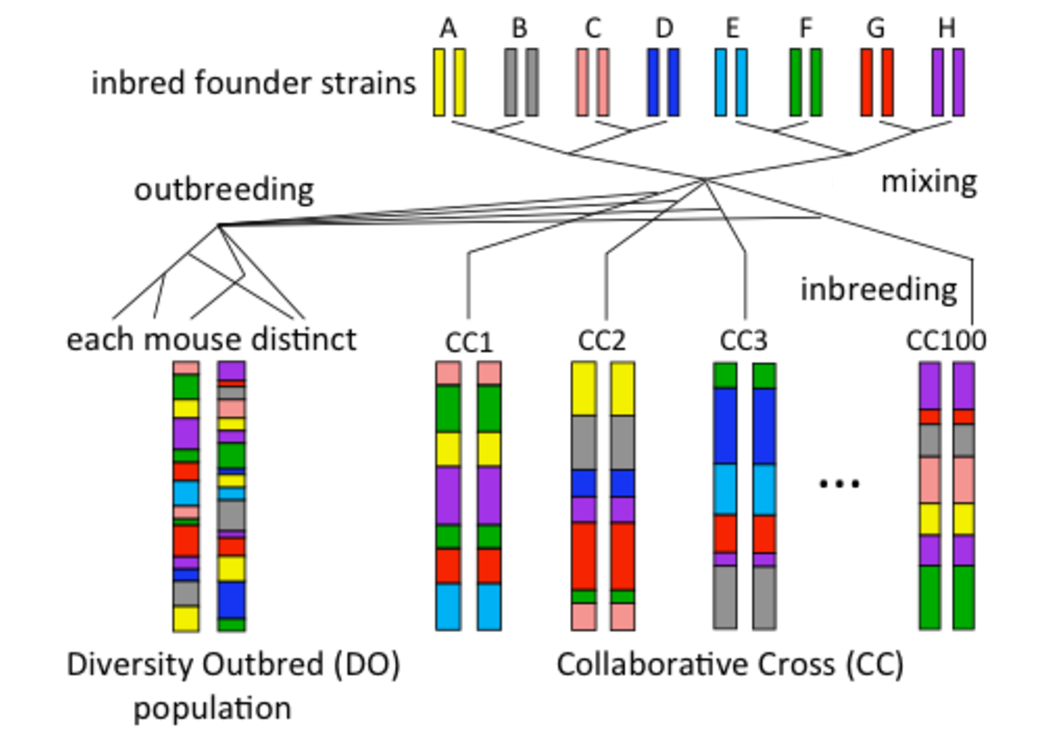
\includegraphics[width=0.7\textwidth, trim={0in 0in 0in 0in}, clip]{figures/1-introduction/cc_and_do.pdf}
\caption[Simplified depiction of the Collaborative Cross and Diversity Outbred stock in mice]{Simplified representations of the CC and DO, with each genome being simplified to a single pair of chromosomes, colored with respect to founder haplotype. The CC is a panel of MPP RI strains. The DO are outbred and have finer-grain founder haplotype blocks than the CC. CC data are analyzed in \textbf{Chapters \ref{chap:hs_rats}} and \textbf{\ref{chap:mediation}}. Figure courtesy of William Valdar. \label{fig:intro_mpp_crosses}}
\end{figure}

\begin{figure}
\centering
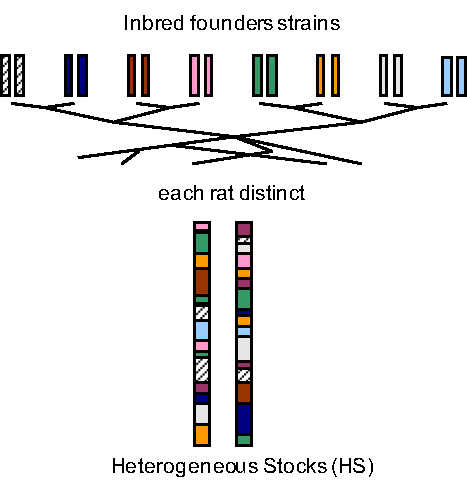
\includegraphics[width=0.5\textwidth, trim={0in 0in 0in 0in}, clip]{figures/1-introduction/hs_cartoon.pdf}
\caption[Simplified depiction of Heterogeneous Stocks]{Simplified representation of the HS, with each genome being simplified to a single pair of chromosomes, colored with respect to founder haplotype. The HS are outbred and have fine-grain founder haplotype blocks, due to many generations of outbreeding. HS populations are similar to the DO (\textbf{Figure \ref{fig:intro_mpp_crosses}}), though likely less balanced in terms of founder haplotype contributions. HS data are analyzed in \textbf{Chapters \ref{chap:mi}} and \textbf{\ref{chap:hs_rats}}. Figure courtesy of William Valdar. \label{fig:hs_cartoon}}
\end{figure}

\subsubsection{Multiparental populations in non-rodent model systems}

Some animal species reproduce rapidly in comparison to rodents, providing the potential for more complex, extensive MPP. Examples in animals include the \textit{Drosophila} Synthetic Population Resource (DSPR) in flies \citep{King2012,King2012a,Long2014,King2017,Najarro2017,Stanley2017}, round worm \citep{Noble2017}, and yeast \citep{Cubillos2017}. Certain plant models can also reproduce prodigiously, as well as being more amenable to inbreeding. Examples of MPP in plants include multiparent advanced generation intercross lines (MAGIC) in \textit{Arabidopsis} \citep{Kover2009,Huang2011} and rice \citep{Bandillo2013,Raghavan2017} and nested association mapping (NAM) populations in maize \citep{Buckler2009}, sorghum \citep{Bouchet2017}, strawberry \citep{Mangandi2017}, and oil palm \citep{Tisne2017}. Though the work presented here will focus completely on data from mice and rats, the ideas and methodology should generalize to these populations as well.

\subsection{Diallel}

The diallel, as a collection of inbred strains and the full set of F1 hybrids, including reciprocal hybrids that distinguish between maternal and paternal strain identities of the parents (A mat $\times$ B pat and B mat $\times$ A pat are reciprocal F1 hybrids with respect to each other), represents an experimental population that is intermediary to bi-parental populations and MPP. Any given individual will descend from at most two inbred strains, but in aggregate, multiple inbred strains are represented. One way to view the diallel with respect to MPP is as the full grid of potential crosses that produce the individuals in the initial outbreeding crosses necessary for the development of an MPP. The diallel is not a mapping population, due to no recombination events between the founder haplotypes; however, it can be used to characterize aggregate strain-level effects on phenotypes \citep{Lenarcic2012}. The diallel will be discussed in greater detail in \textbf{Chapter \ref{chap:didact}}. A simple depiction of the diallel is present in \textbf{Figure \ref{fig:intro_cartoon_diallel}}.

\begin{figure}
\centering
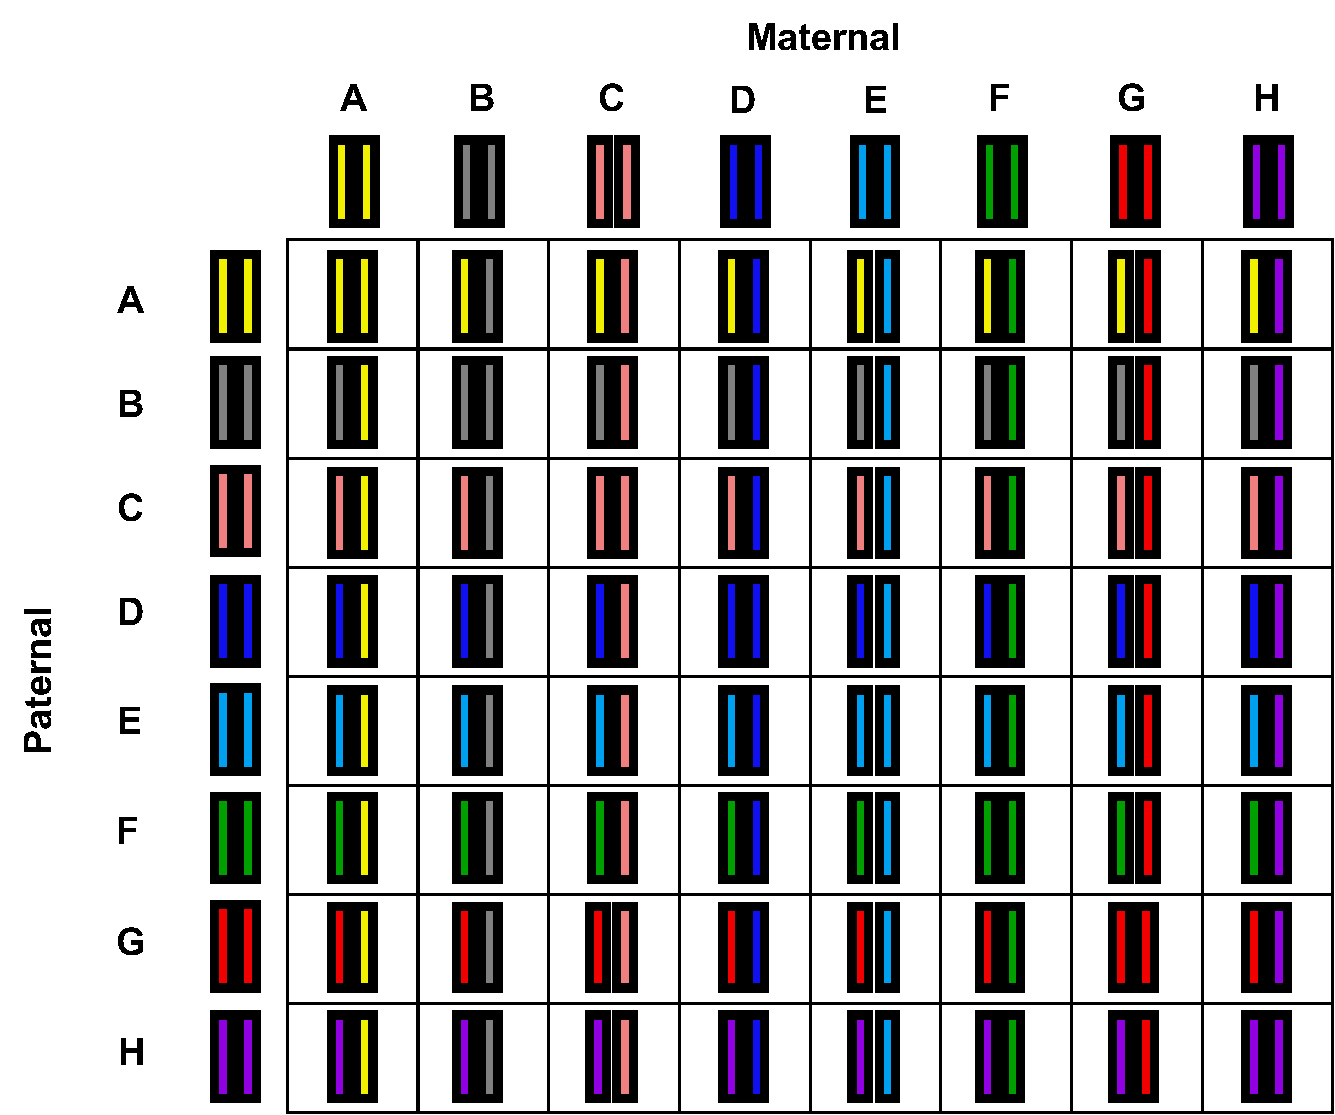
\includegraphics[width=0.8\textwidth, trim={0in 0in 0in 0in}, clip]{figures/1-introduction/diallel_example.pdf}
\caption[Simplified representation of diallel]{Simple representation of a diallel. The paternal strains are listed in the rows, maternal strains in the columns, and the offspring in their intersections. Here a unique genome is presented as a single pair of colored chromosomes. Cells along the diagonal represent the inbred individuals, and the off-diagonal are the F1 hybrids. Cells in mirror positions of each other with respect to the diagonal are reciprocal  F1 hybrids with respect to each other, in which maternal and paternal strains are reversed. The diallel population is not a mapping population because recombination events are not observed between the founder haplotypes. \label{fig:intro_cartoon_diallel}}
\end{figure}

Having described the experimental populations that will be used, the focus now shifts to the primary topics of interest for this dissertation: experimental design and genetic association and related analyses.

\section{Experimental design}

Experimental design is a broad topic, heavily dependent on the specific field of science and its range of experiments. The primary focus will be on the experimental design of QTL mapping experiments, though certain concepts can be extended to other types of experiments. This portion on design is organized into two parts:
\begin{enumerate}
	\item A unique and novel approach to using diallel data as pilot data for selecting bi-parental crosses for QTL mapping (\textbf{Chapter \ref{chap:didact}}).
	\item A focused simulation approach to power calculation for QTL mapping with the realized CC genomes that can assist in choosing the number of strains and replicate observations (\textbf{Chapter \ref{chap:sparcc}}).
\end{enumerate}

\subsection{Diallel-informed bi-parental cross selection}

The selection of a breeding strategy or design for the purpose of QTL mapping has generally involved crossing inbred strains that strongly contrast with respect to the phenotype of interest, as the resulting mapping population should possess segregating variants that influence the phenotype. An Inbred strain survey \citep{Phillippi2014,Rasmussen2014,McMullan2016,Roberts2018} that provides the phenotype information necessary to select promising crosses can be viewed as a partial diallel, thus suggesting that quantitative approaches could be used to leverage information in the diallel for the design of downstream bi-parental crosses. This concept, implemented in an R package called DIDACT (Diallel Informed Decision theoretic Approach for Crosses Tool), is represented in \textbf{Figure \ref{fig:intro_didact_example}}.

\begin{figure}
\centering
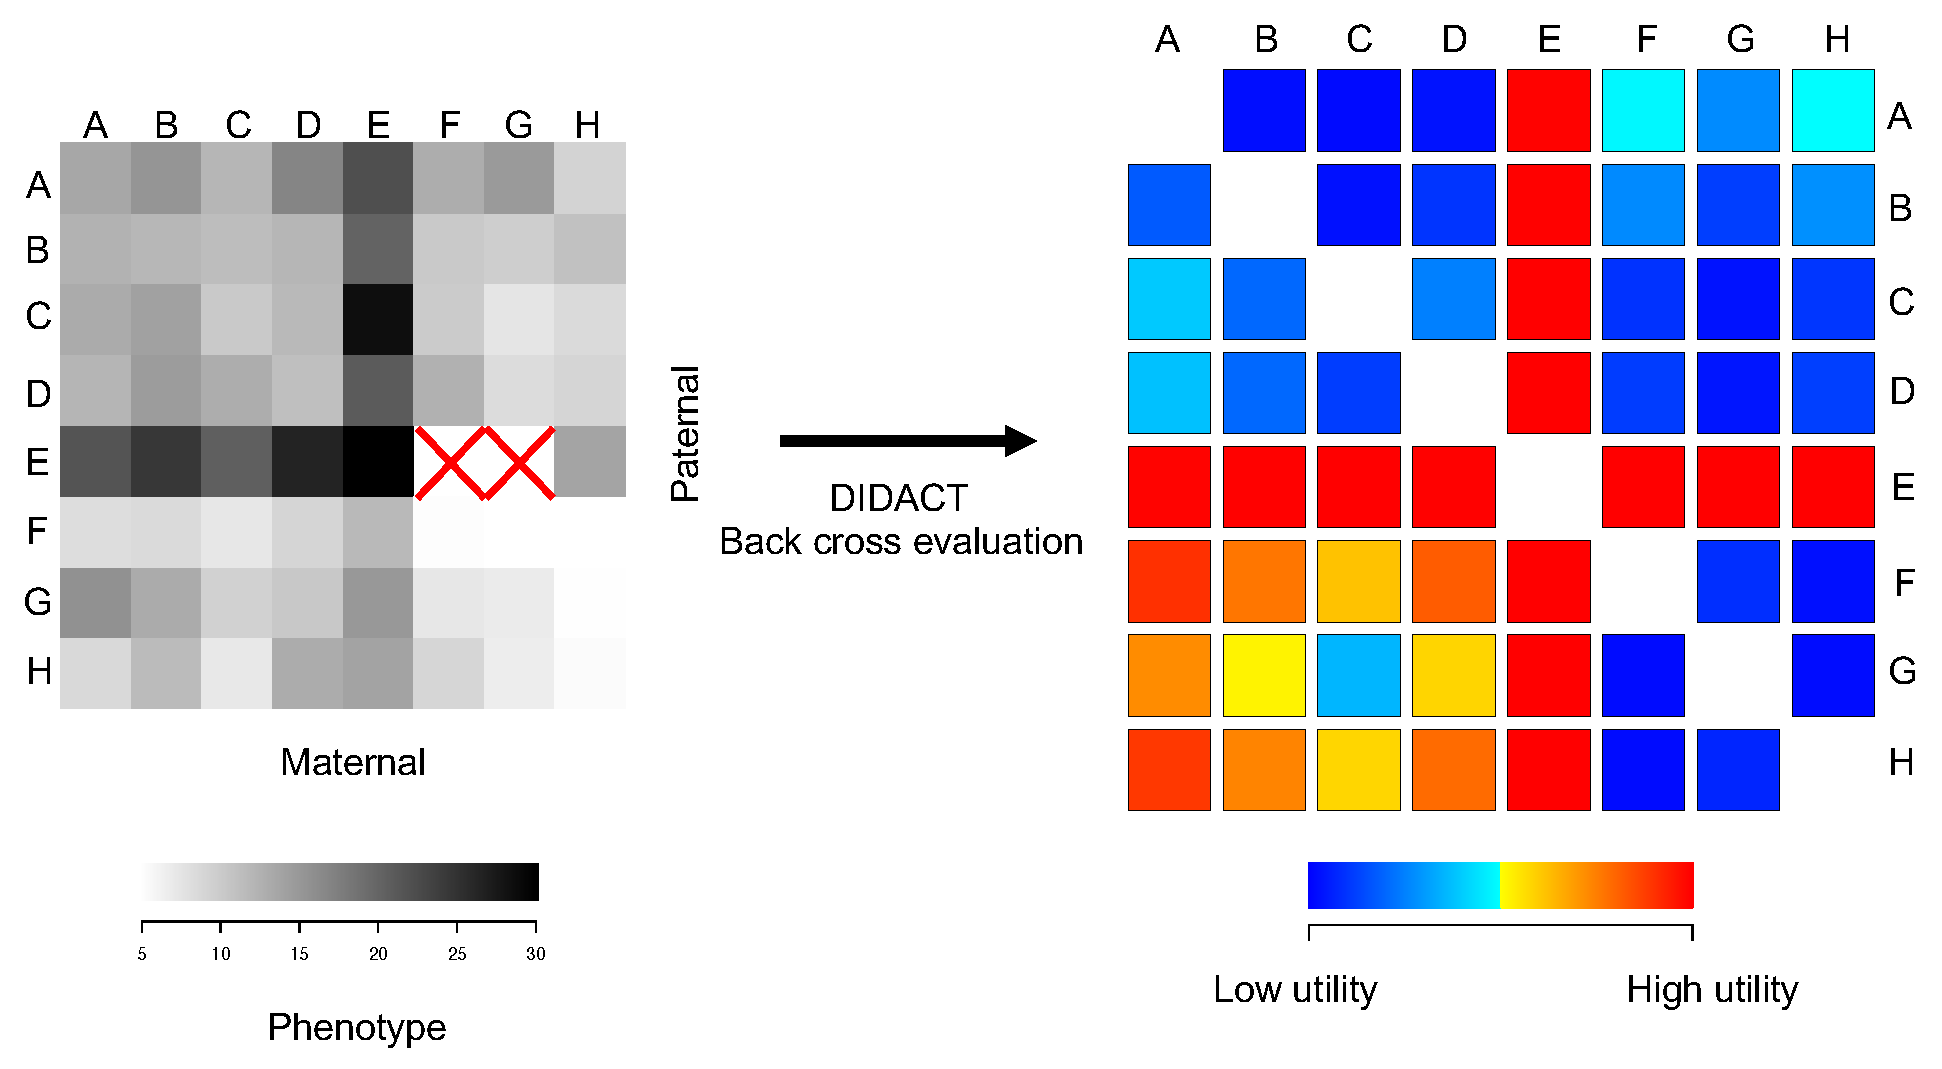
\includegraphics[width=\textwidth, trim={0in 0in 0in 0.1in}, clip]{figures/1-introduction/didact_example.pdf}
\caption[Simplified representation of DIDACT]{DIDACT seeks to evaluate potential bi-parental crosses with respect to a utility function based on pilot data from the diallel. The process involves connecting estimated strain-level effects from the diallel data, represented here as the gray scale grid of mean phenotype level per diallel cell, to a specified utility functions that use these strain-level effect estimates as inputs. A red ``X" indicates that no progeny were produced for that cell of the diallel. In this example, a max utility BC is red and a minimum utility BC is blue. One possible utility function is the power to detect some number of QTL underlying the estimated strain-level effects. Alternatively, a simpler utility function would be the difference in expected phenotype of the progeny based on the strain-level effects. \label{fig:intro_didact_example}}
\end{figure}

\subsubsection{Quantitative analysis of the diallel}

The diallel was originally put forth in the early 20\textsuperscript{th} century, and has seen a steady advancement in methodology, from estimation of general combining ability \citep{Griffing1956} with related F2 populations, to harnessing shrinkage through use of random effects \citep{Zhu1996,Tsaih2005}, and finally the use of Bayesian methods \citep{Greenberg2010,Lenarcic2012}. \cite{Verhoeven2006} explored jointly analyzing a partial diallel with observed downstream F2 populations, and found that such an approach could improve generalizing QTL effects from their narrow F2 mapping population into the broader diallel or panel of inbred strains. 

\subsubsection{DIDACT}

DIDACT (\textbf{Chapter \ref{chap:didact}}) is ignorant of the downstream F2 populations or any mapping populations, and instead seeks to evaluate a specified utility function for each potential downstream cross, which consist of F2, BC, and parent-of-origin effect reciprocal BC, based on strain-level effects as inputs. 

DIDACT is flexible to different utility functions, with one example being the power to map a QTL underlying the estimated strain-level effects. Though the QTL power utility function is dependent on the strong and unlikely assumption that the strain-level effects are attributable to some specified number of QTL, in practice the power tracks with crosses that match strains with contrasting phenotypes. This is similar to what has been done previously, however, now in a principled way that can incorporate complex strain-level effects. Alternatively, utility functions that require less assumptions can be used, such as the expected difference in phenotype based on the strain-level effects, though the utility may be less interpretable in comparison to a quantity like power. More generally, DIDACT is a demonstration of a fundamental Bayesian decision theoretic approach that is extendable to other experimental settings as well.

\subsection{Power to detect QTL in the realized Collaborative Cross}

With \textbf{Chapter \ref{chap:sparcc}}, the focus of the dissertation begins to transition towards genetic association in MPP, though still within the context of experimental design, specifically QTL mapping experiments with the CC. Panels of RI strains are particularly valuable tools for QTL mapping because of their status as GRP, allowing for the potential of QTL results to be replicated across experiments, labs, and related populations \citep{Belknap2001}. Their stable nature as reference populations also allows for highly specific QTL mapping power calculations that can assist researchers in designing efficient but powerful experiments. Previous literature has focused on analytical power estimation within bi-parental RI strains \citep{Kaeppler1997}. Within plant models, QTL mapping power calculations has been performed through simulation, in which both RI genome and phenotype were simulated \citep{Falke2011,Takuno2012}. However, their simulation are tailored for QTL mapping experiments in plants, with particularly large QTL effect sizes and elaborate multiple QTL models, whereas in many phenotypes in animal models, the expectation will be for smaller QTL effects and a preference for single locus models.

\subsubsection{Realized Collaborative Cross}

At the onset of the development of the CC, power calculations were performed through simulations of the RI strain genomes and phenotypes \citep{Valdar2006c}. However, such power estimates are not necessarily representative of the resulting population, which fell short of the stated 1000 goal of RI strains \citep{Churchill2004} due to line extinctions, likely as a result of allelic incompatibilities \citep{Shorter2017}. With the finalized strains (around 75), power calculations can be based on the actual, or realized, CC genomes, and can thus reflect slight deviations from the expected balance in founder contributions \citep{Srivastava2017}.

\subsubsection{SPARCC}

The R package SPARCC (Simulated Power Analysis in the Realized Collaborative Cross) allows for power calculations that can be highly tailored to a specific experiment with a specific set of strains. Alternatively, it can also perform robust power calculations by varying the set of CC strains, the position of the simulated QTL, and even the allelic series \citep{Yalcin2005}. In \textbf{Chapter \ref{chap:sparcc}}, SPARCC is used to investigate how QTL effect size, background strain effect size, number of CC strains, number of replicate observations, and the allelic series affect QTL mapping power in the CC. \textbf{Figure \ref{fig:intro_sparcc_example}} is an example of how SPARCC can interrogate aspects of the experimental design as well as the underlying biology as modulators of QTL mapping power in the CC.

\begin{figure}
\centering
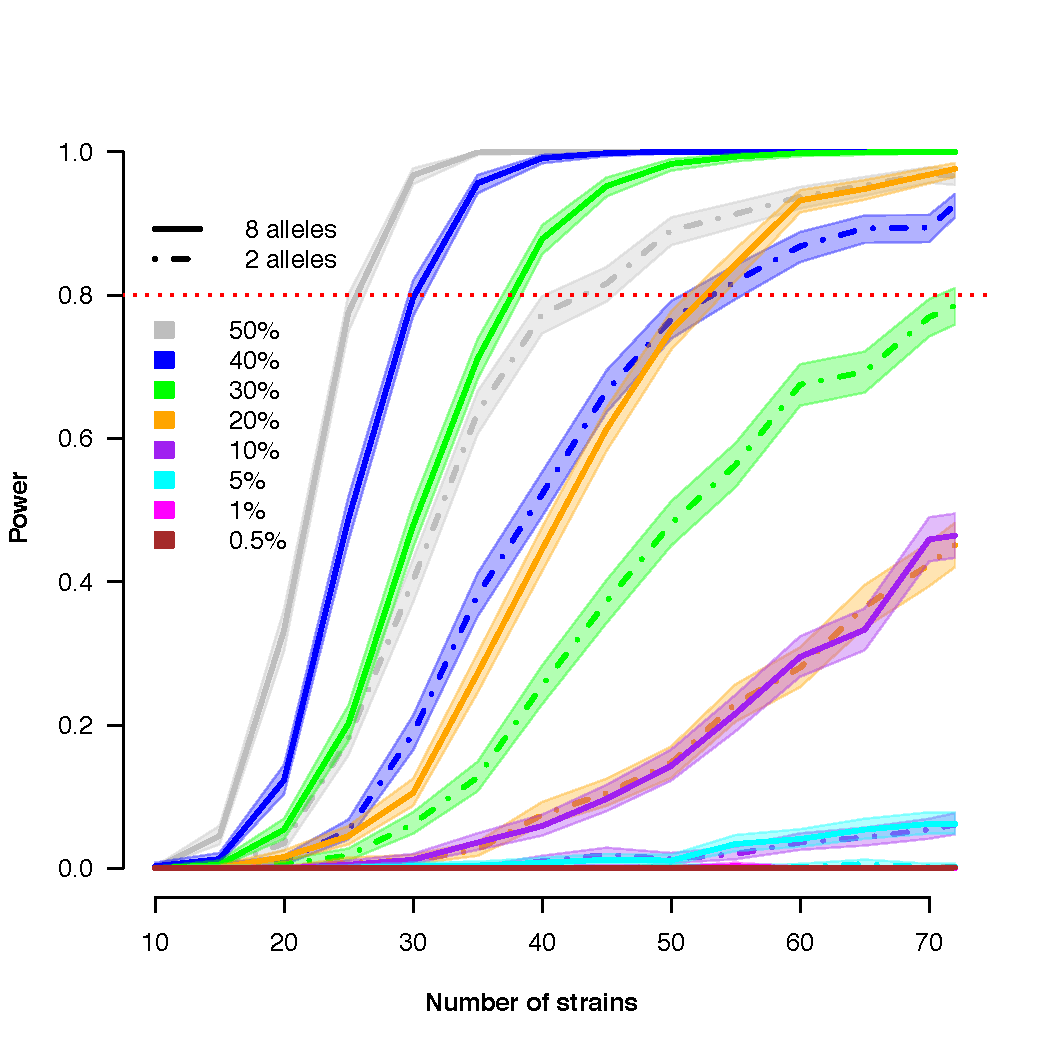
\includegraphics[width=\textwidth, trim={0in 0in 0in 0.1in}, clip]{figures/1-introduction/sparcc_diss_intro.pdf}
\caption[SPARCC power curves comparing eight and two allele models]{Power curves from SPARCC with power on the y-axis and number of CC strains on the x-axis. Five replicate observations per CC strain were simulated for this example. Colors represent different QTL effect sizes in terms of proportion of total variance. Solid lines represent an eight allele model for the simulation, and dashed lines represent an allelic series with two functional alleles. The QTL mapping procedure uses an eight allele alternative model, which is standard practice. Power is significantly worse for allelic series with two functional alleles, mostly due to imbalanced observations of each functional allele. \label{fig:intro_sparcc_example}}
\end{figure}

\section{Genetic association and related analyses}

The focus now shifts fully from experimental design to the actual genetic association analysis in MPP, fine-mapping analyses, and finally a genome-wide mediation approach that statistically integrates multiple levels of data on the same individuals. Specifically, \textbf{Chapters \ref{chap:mi}} focuses entirely on QTL mapping in MPP populations, \textbf{Chapter \ref{chap:hs_rats}} transitions between QTL mapping and fine-mapping approaches to identify candidate variants or genes, particularly emphasizing a mediation approach, and finally \textbf{Chapter \ref{chap:mediation}} is primarily focused on genome-wide mediation in the CC.

In general, QTL mapping approaches developed in simpler bi-parental populations have been extended for use in MPP and been successful \citep{Valdar2006b,Valdar2006a,Valdar2009,Svenson2012,Baud2013,Baud2014,Gatti2014,Phillippi2014}. \textbf{Chapter \ref{chap:mi}} focuses on examples when the use of recycled methods from bi-parental populations can be problematic.

\subsection{Multiple imputation approach to QTL mapping in multiparental populations}

\subsubsection{Developments in interval mapping}

QTL mapping through interval mapping (IM) \citep{Lander1989} models the association between founder haplotype and phenotype, as opposed to the association between a variant genotype and phenotype, as is more common in human GWAS. Founder haplotype identities are not directly observed, but rather probabilistically inferred, commonly with a hidden Markov model (HMM) \citep{Lander1987,Mott2000,Liu2010,Fu2012,Gatti2014,Zheng2015} using genotype data. IM, in its original form, acknowledged this uncertainty through the use of a mixture of Gaussians model \citep{Broman2009}, which required an expectation-maximization (EM) algorithm \citep{Dempster1977} in order to fit maximum likelihood parameters (MLE). The EM is an iterative procedure and thus computationally expensive on a large scale, which becomes more problematic with denser genome scans that involve more tests of association. Additionally, the MLE estimates can be unstable in the presence of little information distinguishing the haplotype states, instead becoming stuck in local maxima. \cite{Haley1992} and \cite{Martinez1992} proposed a computationally efficient regression approximation in which the phenotype is simply regressed on the probabilities, or dosages for an additive model, of the haplotypes. This approximation to IM is sometimes called Haley-Knott (HK) regression or regression-on-probabilities (ROP), and has generally proven accurate, efficient, and thus highly successful. Compared to formal IM, ROP is easily extendible to modeling considerations such as MPP, essentially estimating more allele parameters, as well as other factors such as covariates, and mixed effect models. 

\subsubsection{False associations and problematic uncertainty and founder allele frequency}

Previous work from the Valdar lab has shown that the approximate nature of ROP could produce unstable and uninterpretable regression coefficients, which are often used as allele effect estimates \citep{Zhang2014}, with an extreme example in \textbf{Figure \ref{fig:mi_example}B}. They correct for this issue with the Diploffect model, a Bayesian procedure that involves multiply imputing the haplotype pairs, or diplotypes, from their probabilities. The statistical score of association can also be greatly inflated by the ROP approximation, particularly when at a locus with founder haplotype frequencies that are highly imbalanced, as in \textbf{Figure \ref{fig:mi_example}C}. It is possible that founder haplotypes will be completely lost at random loci simply through genetic drift. If there were no uncertainty, simply no parameter for that founder would be fit at that locus in the genome scan. However, when there is uncertainty, there is the potential that some minute probability mass happens to correlate strongly with the phenotype, resulting in a strong, but artificial, association score, as in \textbf{Figure \ref{fig:mi_example}A}.  

\begin{figure}
\centering
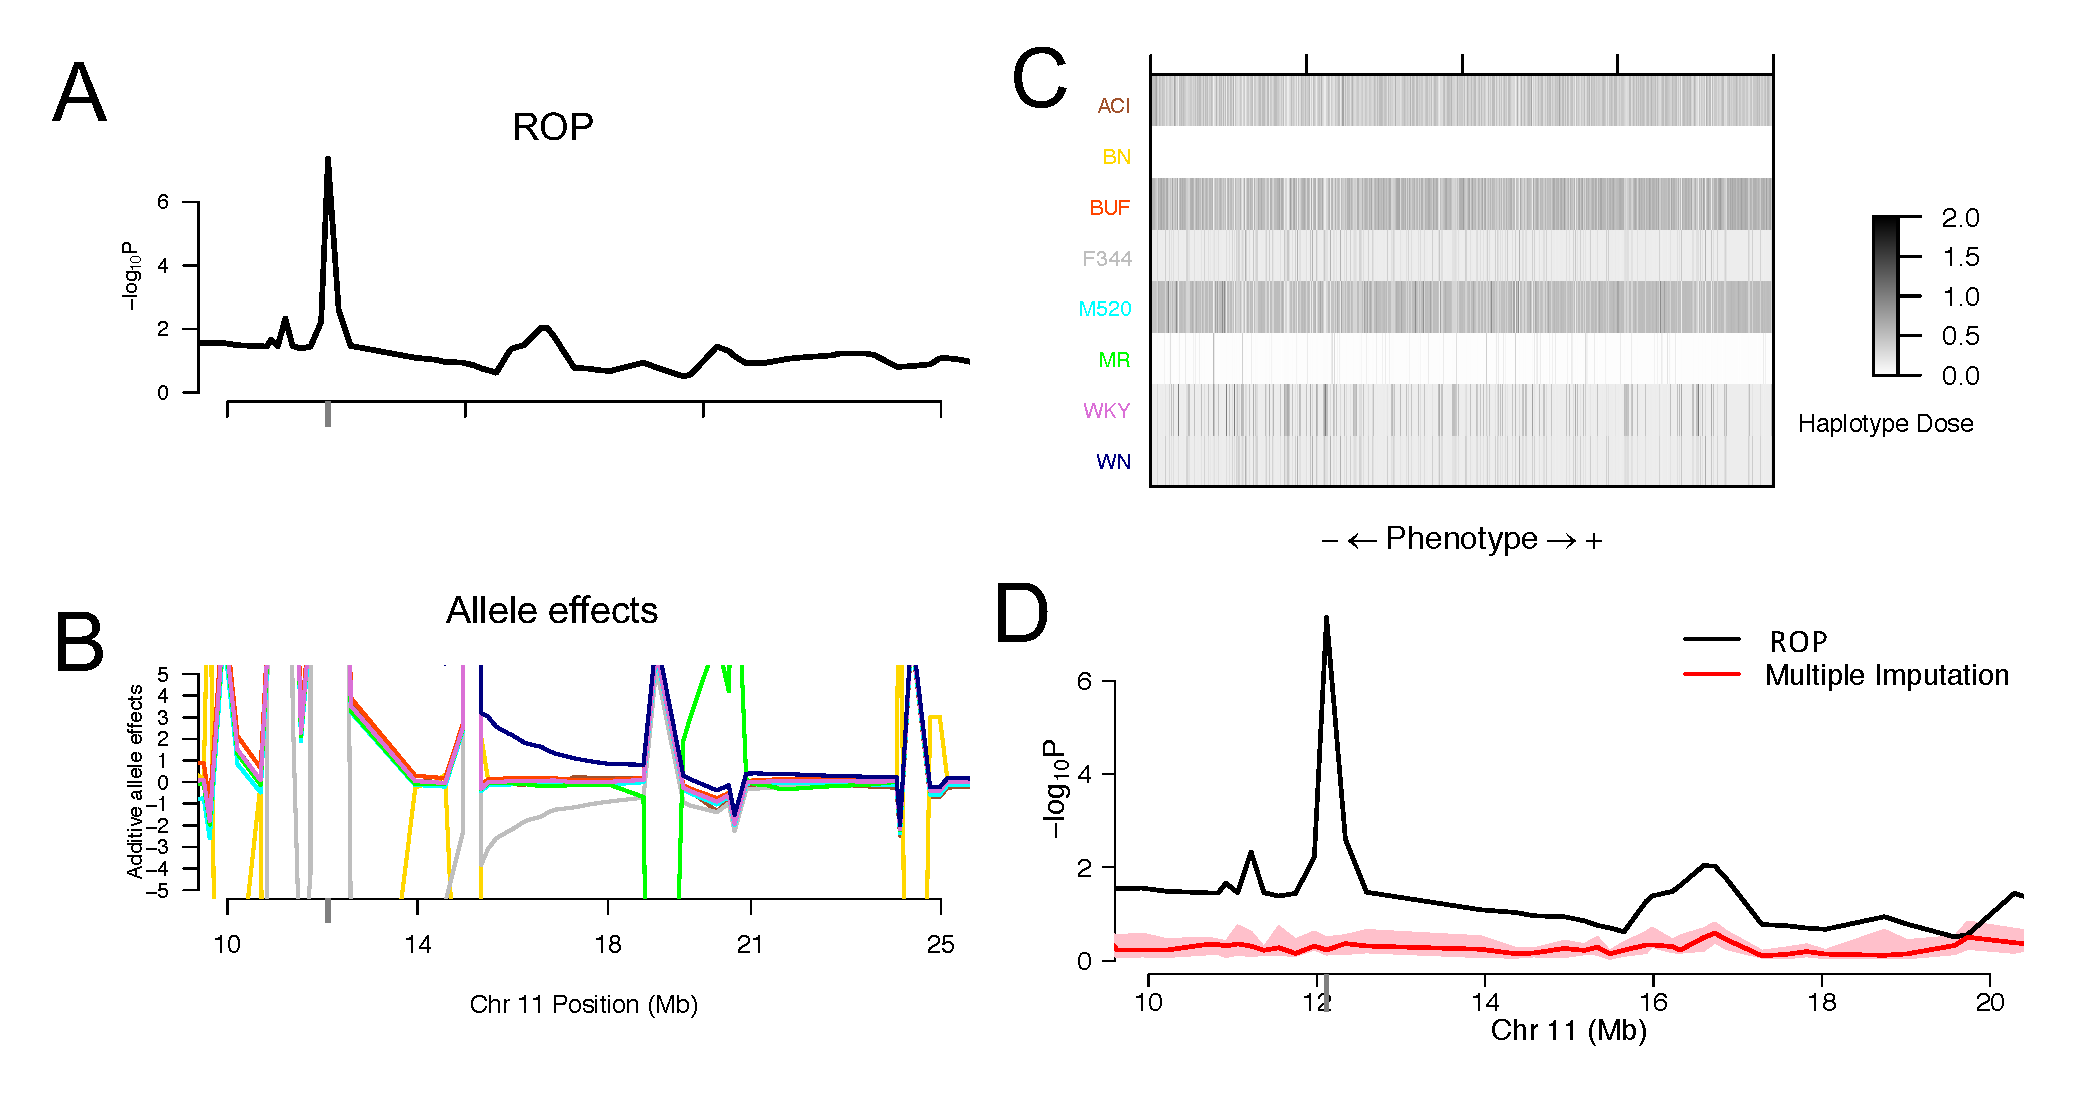
\includegraphics[width=\textwidth, trim={0in 0in 0in 0in}, clip]{figures/1-introduction/mi_example.pdf}
\caption[Example of artificial QTL with ROP]{A surprisingly sharp association signal is observed for a phenotype in a large population ($>700$) of HS rats using ROP (A). The allele effects are highly unstable, particularly around the QTL peak (B). In particular, the BN allele (yellow) appears to approaching negative infinity. A representation of the haplotype dosages at the peak reveals that at the putative QTL there are issues with uncertainty (founders F344, WKY, and WN are largely indistinguishable for many individuals) and imbalance in founder contributions (MR is rarely observed and BN appears to have been lost) (C). A vertical column of the grid represents the haplotype dosage vector of a single rat, with rats being ordered horizontally with respect to phenotype. No substantial founder effects are visually distinguishable, with the extreme BN effect appearing to be an artifact of the problematic uncertainty at the locus. Comparison of ROP (black line) and MI (red line and 95\% confidence interval on the median association across imputations in pink) in the region of the sharp association peak. The signal is completely removed, likely because the BN allele is never sampled. \label{fig:mi_example}}
\end{figure}

\subsubsection{Multiple imputation approach}

There have been Bayesian QTL mapping procedures proposed that also involve multiply imputing the diplotypes from the probabilities \citep{Sen2001,Durrant2010}. \textbf{Chapter \ref{chap:mi}} describes a conservative multiple imputation approach that foregoes a fully Bayesian approach for the sake of computational efficiency. A related problem is also described, in which a founder allele is rarely observed but now with strong certainty. In this situation of unbalanced certain data, shrinkage approaches \cite{Wei2016} should be used, for which two different approaches are discussed. 

Variant association, similar to methods used in human GWAS, is also an alternative to IM, or what could also be called haplotype-based association. Haplotype-based association has some advantages to variant association, such as implicitly modeling a more complex system, such as the local epistasis in the region. However, these strengths are contingent on the stable presence of the various haplotypes, and that they are reasonably estimable. When this is strongly violated, the simpler variant association model can be more stable and powerful, which is a topic of \textbf{Chapter \ref{chap:hs_rats}} and published as \cite{Keele2017}.

\subsection{Analysis of heterogeneous stock rats}

\subsubsection{Imputed SNP association}

The HS rat population that produced the data analyzed in \textbf{Figure \ref{fig:mi_example}} is highly unbalanced with respect to founder haplotype dosage cumulatively across all loci (\textbf{Figure \ref{fig:hs_example}A}). Though haplotype reconstruction poorly distinguished certain founders at some loci, the information content on the simpler SNP genotype can be more complete, resulting in stable association scans (\textbf{Figure \ref{fig:hs_example}B}), and ultimately produced three QTL regions for two different phenotypes, retroperitoneal fat pads (RetroFat) and body weight. The causal variants that induce QTL are usually not obvious, the region instead potentially containing from a handful of genes and variants to hundreds, thus \textbf{Chapter \ref{chap:hs_rats}} also focuses with on quantitative fine-mapping approaches used in order to identify and prioritize candidate genes and variants under the QTL.

\begin{figure}
\centering
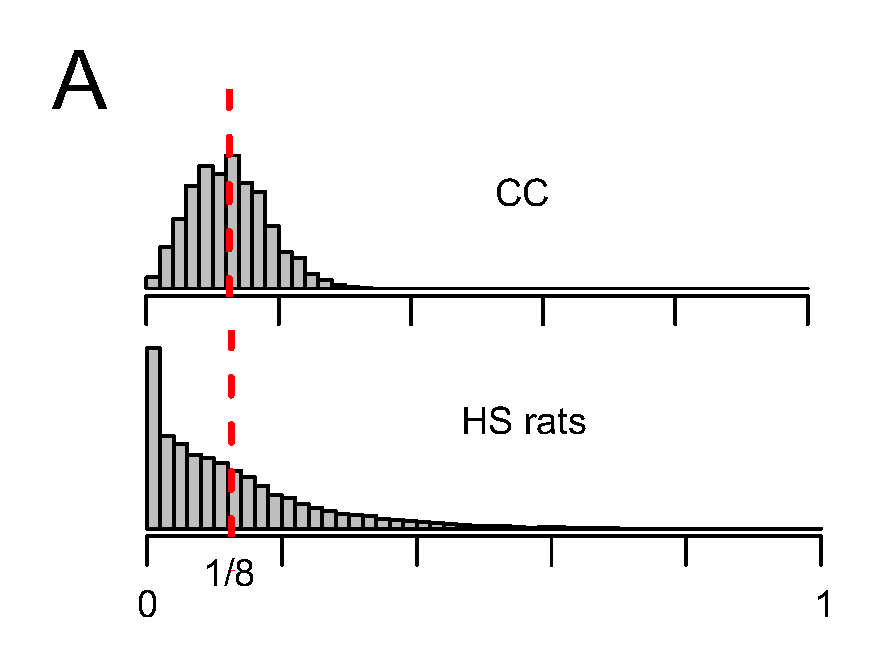
\includegraphics[width=0.7\textwidth, trim={0in 0.1in 0in 0in}, clip]{figures/1-introduction/hs_part1.pdf}
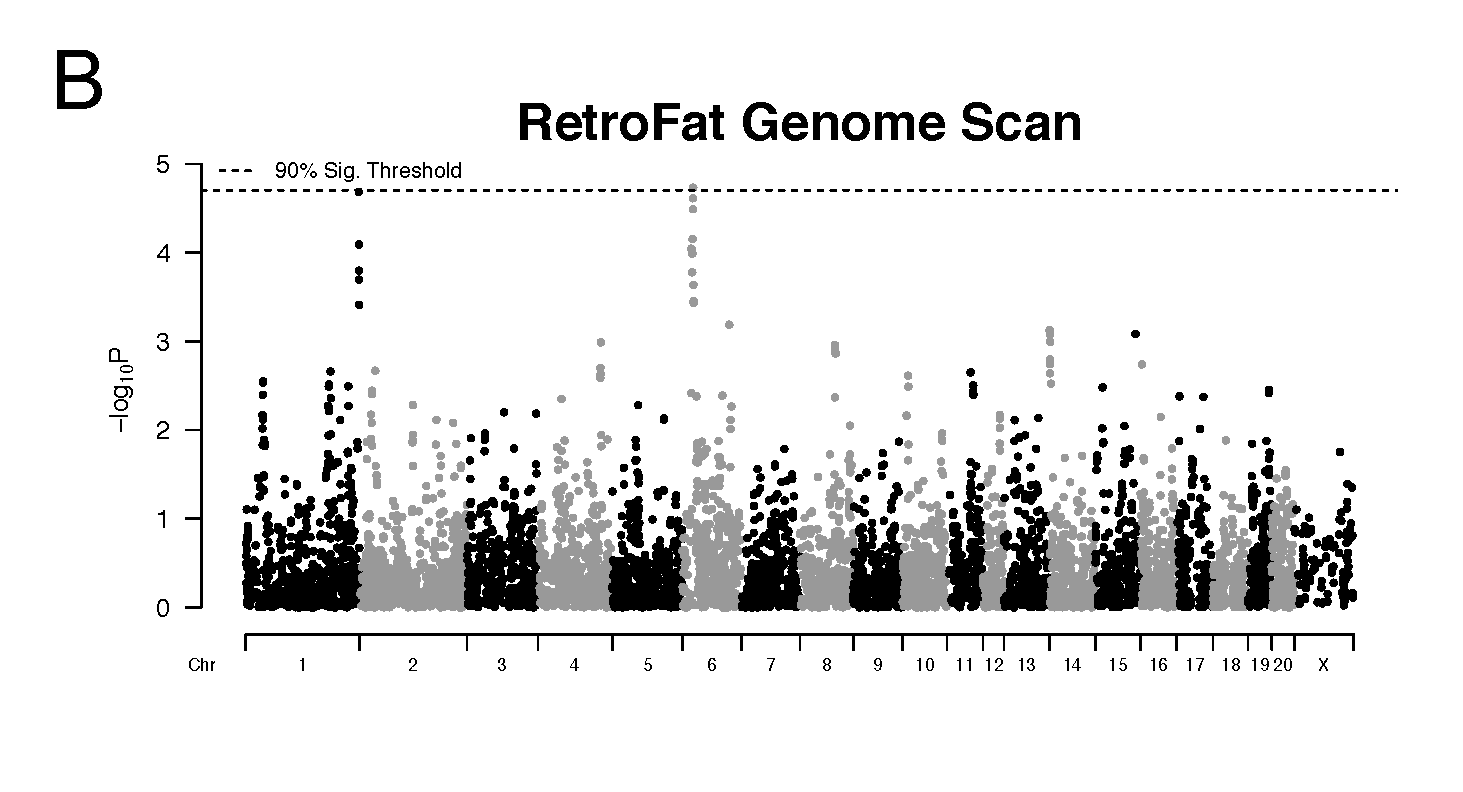
\includegraphics[width=\textwidth, trim={0in 0.4in 0in 0in}, clip]{figures/1-introduction/hs_part2.pdf}
\caption[Example of HS rat analysis]{The histograms of founder haplotype allele frequencies for the CC and the HS rat population (A). The distribution in the CC is centered around 1/8, the expectation for a balanced population descended from eight founders. In contrast, the HS rats, also descended from eight founders, have a large enrichment in small frequencies, particularly near-zero, consistent with the observation that founder haplotypes have been routinely lost at loci across the genome. This pattern of haplotype distribution is problematic to haplotype-based association, a topic discussed in \textbf{Chapter \ref{chap:mi}}. An alternative to the conservative multiple imputation procedure is to impute SNP genotypes from the haplotype probabilities, potentially correcting for genotyping errors and no calls, and do variant association. Whereas there may be poor information to distinguish haplotypes, the simpler SNP imputation may be well-informed, resulting in stabler and more powerful association scans (B). \label{fig:hs_example}}
\end{figure}

\subsubsection{Fine-mapping approaches}

A variety of approaches were used to assess variants within candidate genes that fell in the QTL regions. The Diploffect model \citep{Zhang2014} was used to characterize founder haplotype effects at the QTL, which are useful for potentially identifying variants with alleles that are distributed amongst the founders such that they match these effects patterns. LLARRMA-dawg \citep{Sabourin2015}, a tool designed to simultaneously model and select important SNPs from within a GWAS hit region, significantly reduced a wide QTL region. Protein modeling \citep{Prokop2017} was performed on candidate genes with variants that corresponded with the allele effects and fell within or near the QTL regions to assess the predicted effect of the variant alleles on protein function. Finally, gene expression as a possible mediator of the QTL effect on phenotypes was also investigated.

\subsubsection{Gene expression as mediator of QTL effect on phenotype}

Mediation approaches have recently been applied to genomic data \citep{Battle2014,Chick2016,Roytman2018}, providing avenues for confirming signals as well as potentially teasing apart the underlying relationships between the levels of the biological data. In the context of the HS rats, collaborators collected gene expression data from the liver on a large subset of the sample populations. Only expression levels of genes local to the QTL signal were considered, greatly reducing the computational and testing burden, and a simple model of mediation was used \citep{Baron1986}.

\subsection{Integrative mediation analysis of gene expression and chromatin accessibility}

The latter portion of \textbf{Chapter \ref{chap:hs_rats}} demonstrates a range of ideas as well as quantitative tools for delving further into QTL findings. Mediation, and other causality-oriented approaches such as Mendelian Randomization \citep{Smith2003,Lawlor2008}, represent exciting areas of research that leverage the big data that are being collected, with multiple dimensions per individual, sometimes referred to as multi-omics, to answer questions about and better understand the relationships between the levels of data, with particular focus on the relationships at play in the flow of information from gene to phenotype \citep{Degner2012,Pai2015,Battle2015,Alasoo2017,Wu2018}. \textbf{Chapter \ref{chap:mediation}} further explores this topic, by investigating genetic regulation of gene expression and chromatin accessibility, as well as the potential relationship between them, genome-wide, in CC mice through an integrative mediation analysis.

\begin{figure}
\centering
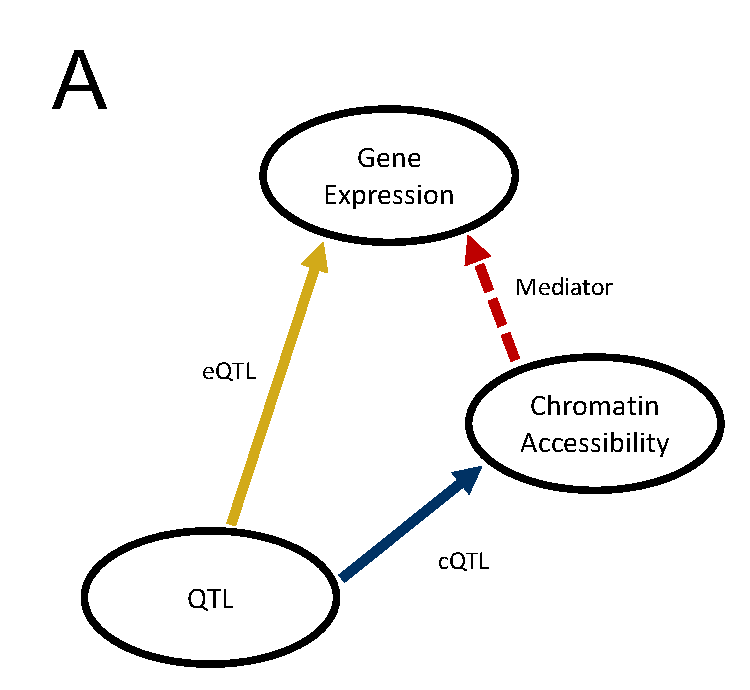
\includegraphics[width=0.7\textwidth, trim={0in 0.1in 0in 0in}, clip]{figures/1-introduction/mediation_example_part1.pdf}
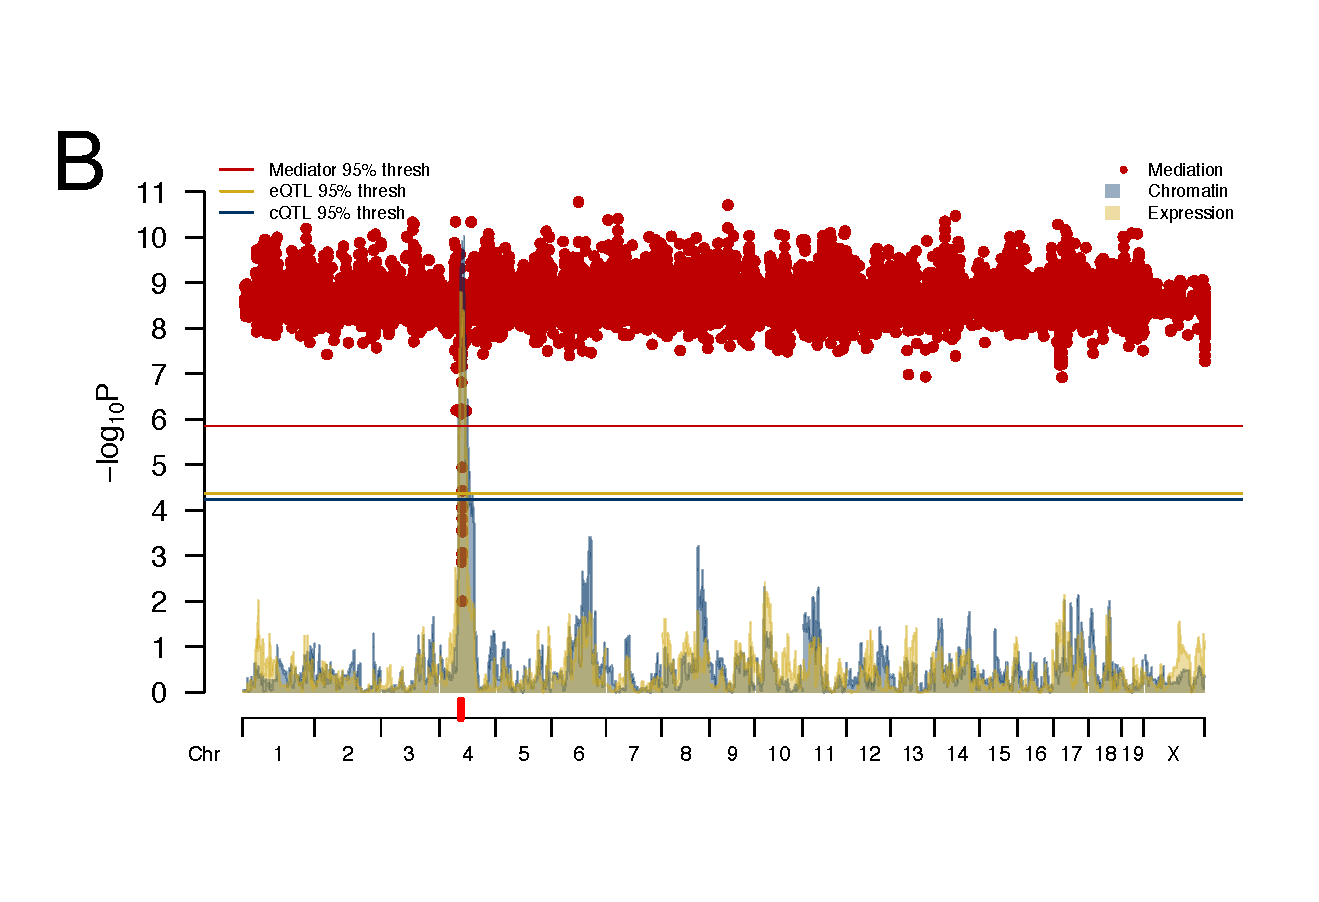
\includegraphics[width=\textwidth, trim={0in 0.9in 0in 0in}, clip]{figures/1-introduction/mediation_example_part2.pdf}
\caption[Mediation model and example of genome-wide significant mediation of gene expression through chromatin accessibility]{The simplistic model of chromatin accessibility as a possible mediator of the eQTL effect on gene expression (A). This model was tested for all genes with detected eQTL in lung, liver, and kidney tissue for 47 CC strains with only a single observation per strain. Example of genome-wide significant mediation (B). The gene \textit{Alad} has a significant eQTL, local to its transcription start site (TSS) (yellow) on chromosome 4, in kidney tissue. The chromatin accessibility in the region also has a significant local cQTL (blue). Significant mediation is detected in the area (red), by the drop in p-value that reflects chromatin accessibility out-competing the eQTL when included in the null and alternative models of the genome scan of \textit{Alad} expression. \label{fig:mediation_example}}
\end{figure}

\subsubsection{Description of CC data and analyses}

This project is highly collaborative with members of the Furey Lab, as well as collaborators at Texas A\&M (Ivan Rusyn) and NC State (Fred Wright) and the results are preliminary. As such, the description in \textbf{Chapter \ref{chap:mediation}} will be brief, and focus on the methodology, which relates to the research focus of this dissertation. The data for these analyses consist of RNA-Seq (gene expression) and ATAC-Seq (chromatin accessibility) in three tissues (lung, liver, and kidney) for only 47 CC strains with a single observation per strain. QTL mapping through a multi-stage conditional fitting approach \citep{Jansen2017} was performed for both expression (eQTL) and chromatin accessibility (cQTL) in each tissue, allowing for the potential of multiple QTL per phenotype. A genome-wide mediation analysis was developed and used that draws from the approach used in \cite{Chick2016} for jointly modeling gene expression and protein levels. Despite mediation not being equivalent to causality and the undoubtedly complex and multifactorial nature of the underlying biology involved in the steps of the regulation of the flow of information from genomic DNA to protein, simplistic mediation models can detect evidence that is consistent with broad hypotheses of how the levels relate. MPP, such as the CC or DO, can be particularly powerful tools for these genome-wide mediation approaches due to the ability to characterize associations with respect to the founder haplotypes (allele effects), and potentially replicate findings or design downstream experiments in related populations.

\section{Summary}

This dissertation describes a range of methods and analyses for use with MPP. \textbf{Chapters \ref{chap:didact}} and \textbf{\ref{chap:sparcc}} describe approaches for designing experiments, first using MPP pilot data in the form of the diallel to select promising bi-parental crosses, and second to design adequately powered mapping studies of the finalized CC strains. \textbf{Chapters \ref{chap:mi}}, \textbf{\ref{chap:hs_rats}}, and \textbf{\ref{chap:mediation}} collectively focus on genetic association analyses for MPP: QTL mapping in MPP populations with problematic founder haplotype uncertainty, imputed SNP association and fine-mapping approaches in an HS rats population, and an integrative genetic mediation analysis of gene expression and chromatin accessibility in the CC, respectively. Taken together broadly, this research presents novel methodologies for accommodating and thus harnessing MPP resources for powerful genetic experiments.



